\documentclass[12pt,a4paper]{report}
\usepackage[utf8]{inputenc}
\usepackage[english,russian]{babel}
\usepackage{indentfirst}
\usepackage{pdfpages}
\usepackage{titlesec}
\usepackage{listings}
\usepackage{amsmath}

% Вставка картинки
\usepackage{graphicx}
\graphicspath{{schemes/}}
\DeclareGraphicsExtensions{.pdf,.png,.jpg}

\usepackage[tableposition=top,singlelinecheck=false]{caption}

\usepackage[14pt]{extsizes}

\newcommand{\hsp}{\hspace{20pt}}
\titleformat{\chapter}[hang]{\large\bfseries}{\thechapter{. }}{0pt}{\large\bfseries}
\titlelabel{hlabel-formati}
\titlespacing{\chapter}{42pt}{-20pt}{12pt}
\titleformat{\section}[hang]{\large\bfseries}{\thesection{. }}{0pt}{\large\bfseries}
\titlespacing{\section}{42pt}{12pt}{5pt plus 5pt}

% Отступ абзаца
\usepackage{indentfirst}
\setlength{\parindent}{1.5cm}

% Межстрочный интервал
\usepackage{setspace}
\onehalfspacing % интервал 1.5


\usepackage{csvsimple}

\bibliography{biblio}
\lstset{frame=none, tabsize=4}

\usepackage[left=3cm, right=1cm, top=2cm, bottom=2cm]{geometry}

\AtBeginDocument{%
	\renewcommand\contentsname{Содержание}
}

\begin{document}
	% Титульник
	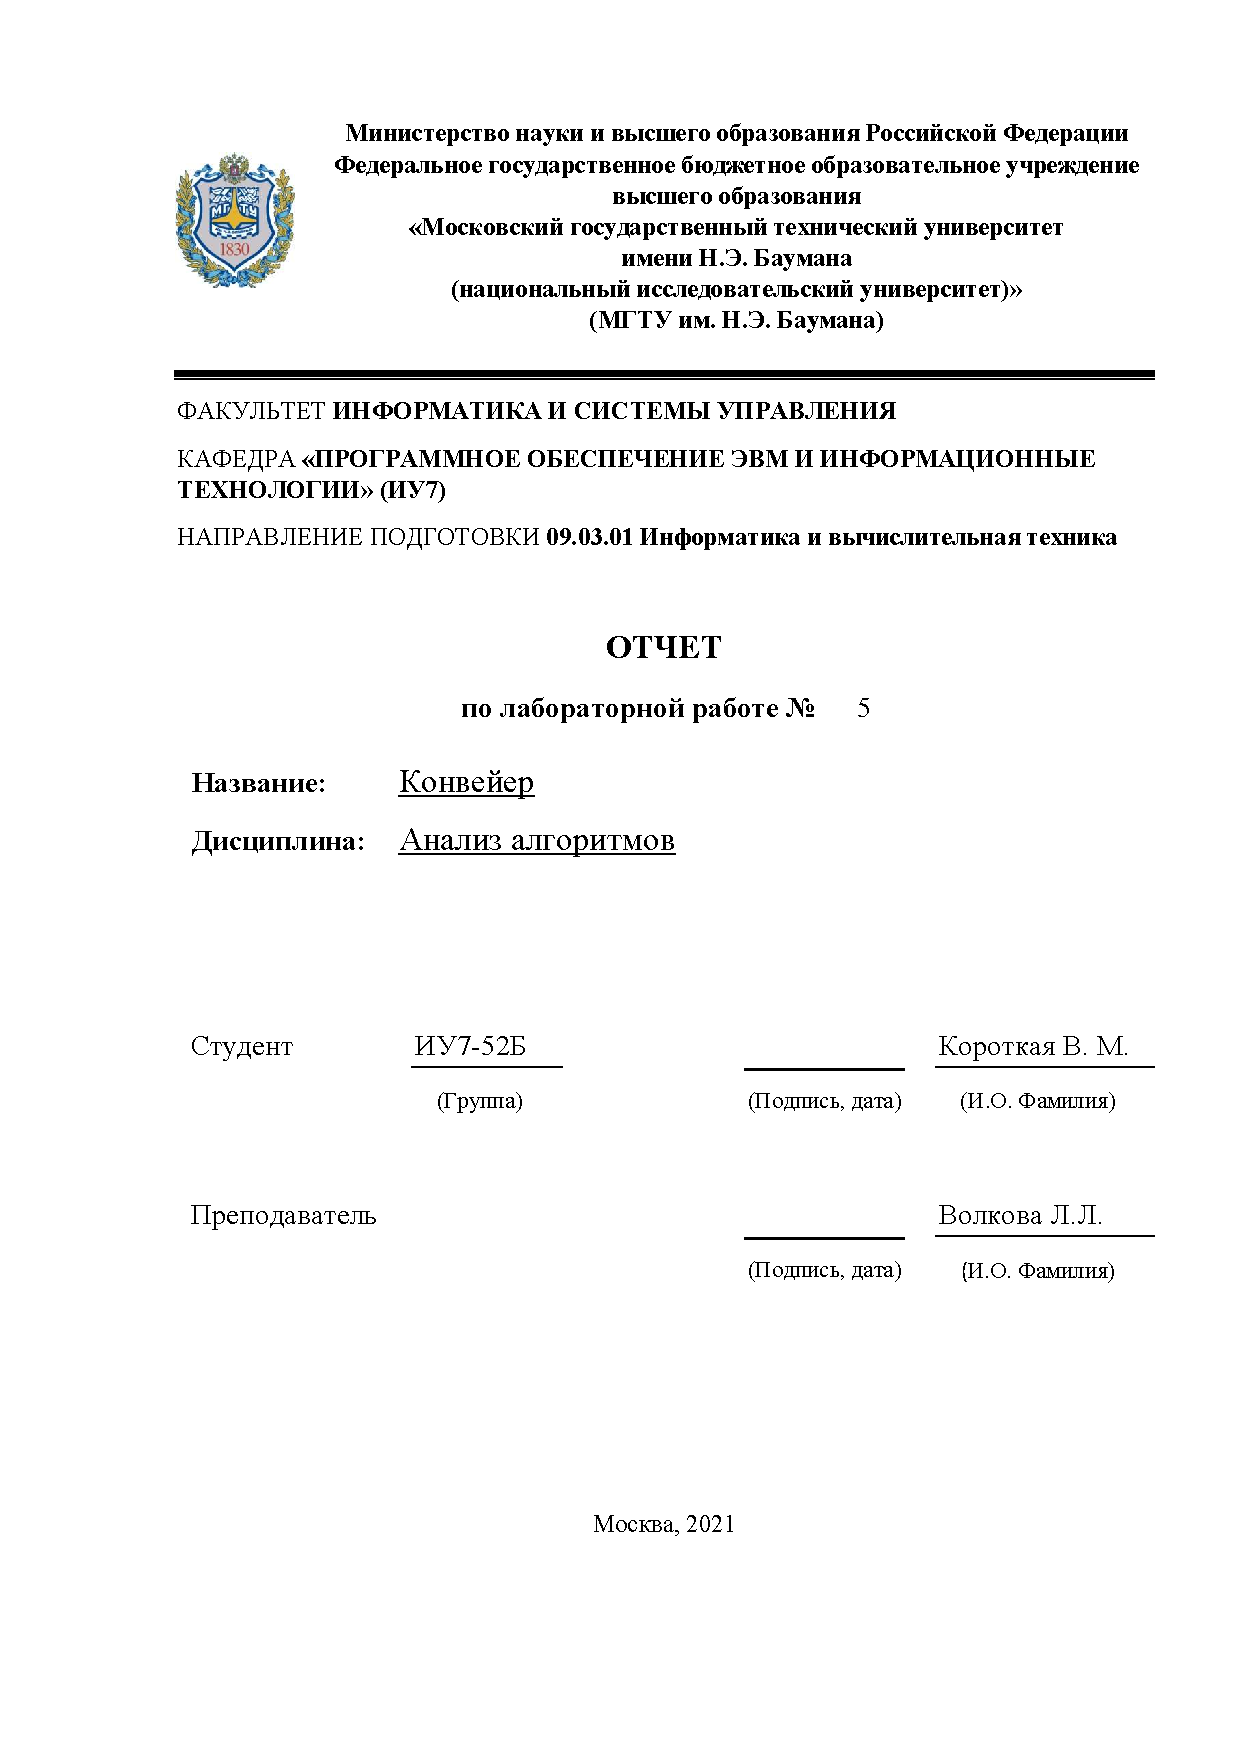
\includepdf[pages=1]{titul.pdf}
	% Оглавление
	\tableofcontents


\newpage
\chapter*{Введение}
\addcontentsline{toc}{chapter}{Введение}

КОНВЕЙЕР - (англ. сonveyеr, от сonvey – продвигать, перевозить) (транспортёр), машина непрерывного действия, служащая для перемещения сыпучих, кусковых, штучных и др. грузов. 

Историческая справка

Машины непрерывного действия были известны уже в глубокой древности – за неск. тысячелетий до н. э. Подъёмники с ковшами применяли для водоснабжения и в системах орошения, при строительстве укреплений, на рудниках. В Древнем Египте и в Китае использовали водоподъёмные машины, а также устройства с толкающими скребками, винтом. В Зап. Европе в 16–17 вв. дерев. винтовые К. устанавливали на мукомольных предприятиях.

Разработчики архитектуры компьютеров издавна прибегали к методам проектирования, известным под общим названием "совмещение операций", при котором аппаратура компьютера в любой момент времени выполняет одновременно более одной базовой операции. Этот общий метод включает два понятия: параллелизм и конвейеризацию. Параллелизмы был рассмотрен в предыдущей работе.
Сейчас время конвейера.



Цель данной работы - разработка и исследование конвейерных вычислений.

Для достижения данной цели необходимо рассмотреть следующие задачи:
\begin{itemize}
	\item описать конвейерную обработку и применение ее на практики;
	\item реализовать конвейерную обработку на примере шифрования строк;
	\item провести экспериментальные замеры времени реализованного конвейера.
\end{itemize}

\newpage
\chapter{Аналитическая часть}

В данном разделе рассматривается понятие конвейерной обработки.
Так же рассматривается описание решаемой задачи в лабороторной работе.

\section{Конвейерная обработка}

Конвейеризация (или конвейерная обработка) в общем случае основана на разделении подлежащей исполнению функции на более мелкие части, называемые ступенями, и выделении для каждой из них отдельного блока аппаратуры. Так обработку любой машинной команды можно разделить на несколько этапов (несколько ступеней), организовав передачу данных от одного этапа к следующему. При этом конвейерную обработку можно использовать для совмещения этапов выполнения разных команд. Производительность при этом возрастает благодаря тому, что одновременно на различных ступенях конвейера выполняются несколько команд. Конвейерная обработка такого рода широко применяется во всех современных быстродействующих процессорах.

\section{Алгоритмы шифрования строк}

Идея шифрования строк - преобразование их для скрытия от посторонних. В то же время,  те которым предназночается информация способны ее дешифровать.

В лабораторной работе будут реализованы шифры Цезаря и Вернама (XOR - шифр).

Шифр Цезаря - имеется ключ в виде числа от 1 до 25 (для латиницы) и каждая буква строки смещаеться на значение равное ключу.

Шифр Вернама (XOR - шифр) - строка разбивается на отдельные символы и каждый символ представляется в бинарном виде. Далее с каждым символом применяется операция XOR с ключом. В итоге получаем зашифрованную строку.

\section*{Вывод}
В данном работе стоит задача реализации ассинхронных конвейерных вычислений. Были рассмотрены особенности построения конвейерных вычислений.

Входными данными является строка.

Выходными данными является зашифрованная строка.

На программу накладываюся следующие ограничения:
\begin{itemize}
	\item строка не должна быть пустой.
\end{itemize}


\newpage
\chapter{Конструкторска часть}

В данном разделе будут приведены схемы алгоритмов шифрования и модель вычислений.

\section{Схемы}

\begin{figure}[ht]
	\center{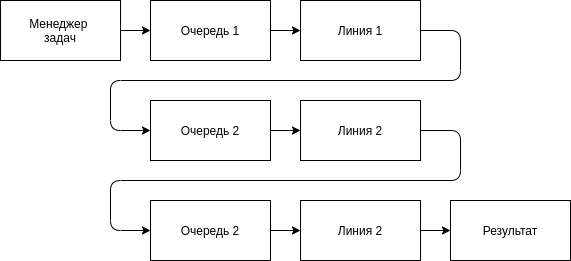
\includegraphics[scale=0.6]{conveyer}}
	\caption{Схема организации конвейерных вычислений.}
	%\label{fig:image}
\end{figure}

\section{Структура ПО}

\begin{figure}[ht]
	\center{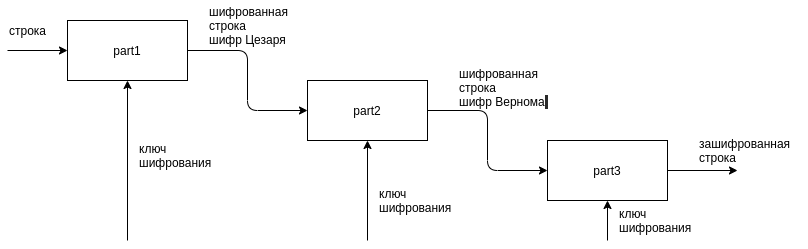
\includegraphics[scale=0.6]{idef0}}
	\caption{idef0 - диограмма конвейера.}
	%\label{fig:image}
\end{figure}

\section{Схемы}



%\section{Описание структур данных}

Для реализации конвейерных вычислений, введем пользовательские типы данных:
\begin{itemize}
	\item struct Request - описывает результат обработки задачи на конвейерной ленте
\end{itemize}

\begin{lstlisting}[frame=single, numbers=left]
struct Request{	
	double timeS[3];
	double timeE[3];
	
	std::string dataStr;
	int len, num;
};	
\end{lstlisting}

Здесь:
\begin{itemize}
	\item timeS[3] - массив, содержащий время начала обработки строки на каждой ленте;
	\item timeE[3] - массив, содержащий время окончания обработки строки на каждой ленте;
	\item dataStr  - строка, переданная для обработки;
	\item len      - длина строки;
	\item num      - номер заявки.
\end{itemize}

\section*{Вывод}
На основании теоритических данных была построена схема организации конвейерных вычислений на примере конвейера с тремя лентами.

Так же приведено описание пользовательских структур данных.
\newpage
\chapter{Технологическая часть} 

В данном разделе приведены средства реализации, требования к ПО и листинги кода.

\section{Средства реализации}
В качестве языка программирования был выбран с++. Данный язык знаком и предостовляет все необходимые ресурсы.
В качестве среды разработки я использовала Visual Studio Code, т.к. считаю его достаточно удобным и легким.
Visual Studio Code подходит не только для  Windows, но и для Linux, это еще одна причина, по которой я выбрала VS code, т.к. у меня установлена ОС  fedora 34.

\section{Сведенья о модулях программы}

Данноя программа разбита на модули:

\begin{itemize}
	\item main.cpp - файл, содержащий точку входа в программу;
	\item conveyor.cpp - файл, содержащий реализацию конвейера.
\end{itemize}


\section{Реализация конвейера}

\noindent\textrm{Листинг 3.1: Функция запускающая конвейер.}
\begin{lstlisting}[frame=single, numbers=left]
void Conveyor::run()
{
    generateRequest();
	
    std::thread t1 = std::thread(&Conveyor::part1, this);
    std::thread t2 = std::thread(&Conveyor::part2, this);
    std::thread t3 = std::thread(&Conveyor::part3, this);
	
    t1.join();
    t2.join();
    t3.join();
}	
\end{lstlisting}

\noindent\textrm{Листинг 3.2: 1 Лента - шифр Цезаря.}
\begin{lstlisting}[frame=single, numbers=left]
void Conveyor::part1()
{
    for(; ft1 < ntask; ft1++)
    {
        Request *req;
		
        if (startQ.size())
        {
            req = startQ.front();
            startQ.pop();
        }
        else continue;
		
        req->timeS[0] = clock();
        req->cryptCaesar(12);
        req->timeE[0] = clock();

        m1.lock();
        q2.push(req);
        m1.unlock();
    }
}

\end{lstlisting}

\noindent\textrm{Листинг 3.3: 2 Лента - шифр Вернама.}
\begin{lstlisting}[frame=single, numbers=left]
void Conveyor::part2()
{
    while(q2.size() == 0)
        continue;
	
    for (; ft2 < ntask; ft2++)
    {
        while(q2.size() == 0)
            continue;
		
        Request *req;
		
        m1.lock();
		
        req = q2.front();
        q2.pop();
		
        m1.unlock();
		
        req->timeS[1] = clock();
        req->cryptXor('p');
        req->timeE[1] = clock();
		
        m2.lock();
        q3.push(req);
        m2.unlock();
    }
}	
\end{lstlisting}


\noindent\textrm{Листинг 3.4: 3 Лента - шифр Вернама..}
\begin{lstlisting}[frame=single, numbers=left]
void Conveyor::part3()
{
    while(q3.size() == 0)
        continue;
	
    for(; ft3 < ntask; ft3++)
    {
        while (q3.size() == 0)
        continue;
		
        Request *req;
		
        m2.lock();
		
        req = q3.front();
        q3.pop();
		
        m2.unlock();
		
        req->timeS[2] = clock();
        req->cryptXor('a');
        req->timeE[2] = clock();
		
        result.push_back(req);
    }
}	
	
	
\end{lstlisting}	

\section*{Вывод}
В данном разделе был реализован выше описанный алгоритм шифрования. Разработано программное обеспечение, представленны листинги программы.

\newpage
\chapter{Исследовательская часть} 

В данном разделе будет произведено измерение временных характеристик.

\section{Технические характеристики}

\begin{figure}[ht]
	%\center{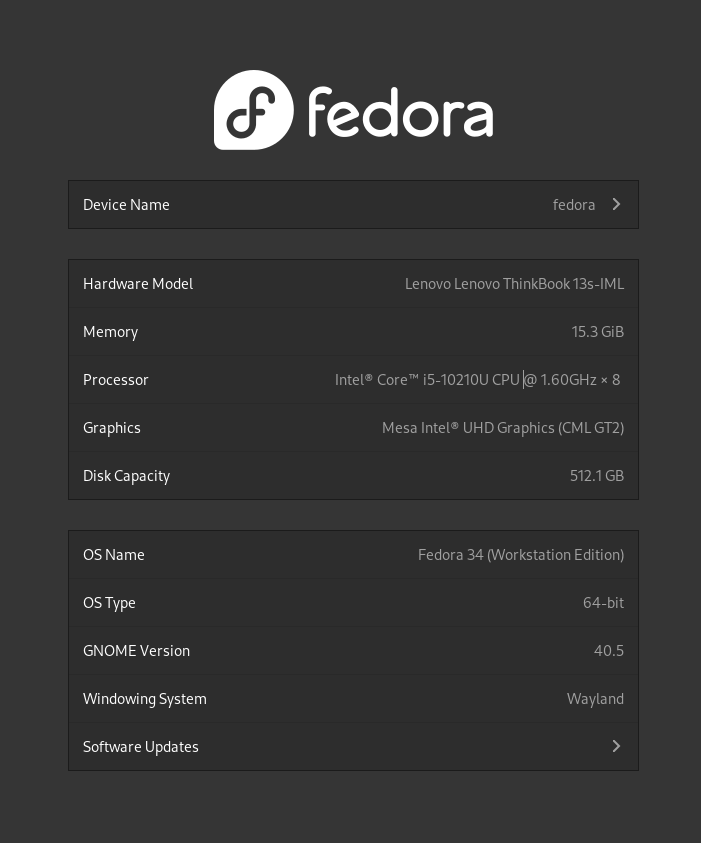
\includegraphics[scale=0.6]{texn}}
	%\caption{}
	%\label{fig:image}
\end{figure}

Технические характеристики устройства на котором выполнялось исследование:
\begin{itemize}
	\item процессор Intel® Core™ i5-10210U CPU @ 1.60GHz × 8;
	\item память 15.3 GiB;
	\item операционная система Fedora 34 (Workstation Edition) 64-bit.
\end{itemize}

Исследования проводились на ноутбуке включенном в сеть электропитания. Во время тестирования ноутбук был нагружен приложениями окружения рабочего стола, а так же системой тестирования.

\section{Временные характеристики}

Замеры времени проводились на конвейере, обрабатывающем 200 заявок, каждая из которых содержит строку 
длинной 1000000 символов. 
Было замерено время 20 конвейеров, приведены усреднённые результаты.\\

На графиках 4.1 - 4.2 представлены результаты замеров времени во 2 и 3 очередях, и общее время,
проведённое заявкой во всей системе, где t в миллисекундах.

\begin{figure}[h!]
	\center{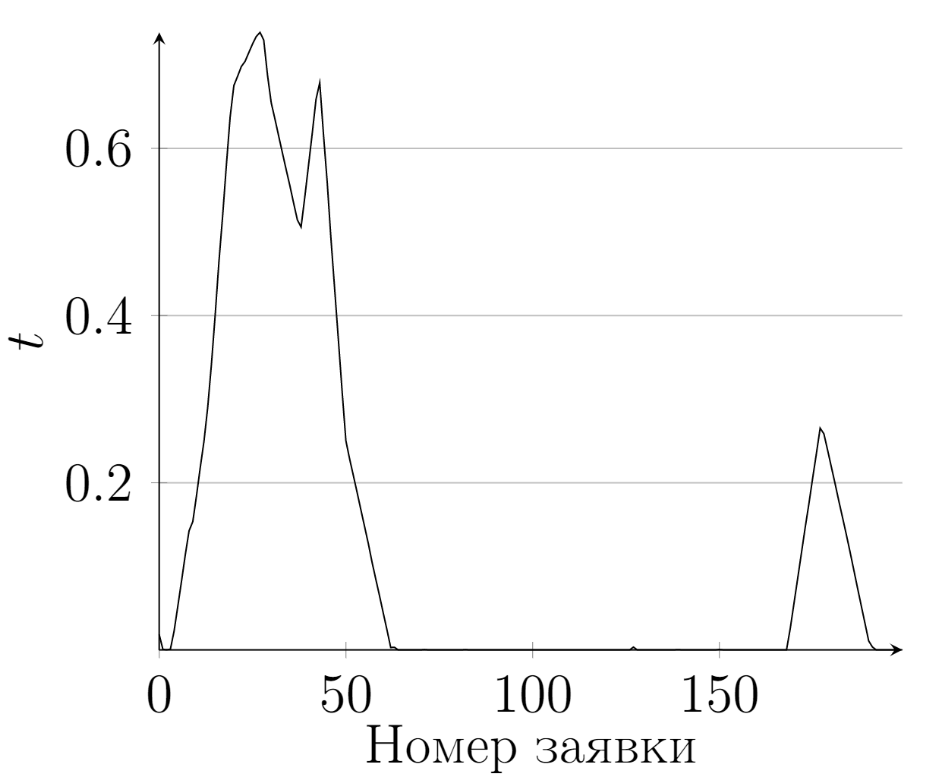
\includegraphics[scale=0.5]{graph_2q.png}}
	\caption{время проведённое заявкой во второй очереди}
	\label{fig:image}
\end{figure}

\begin{figure}[h!]
	\center{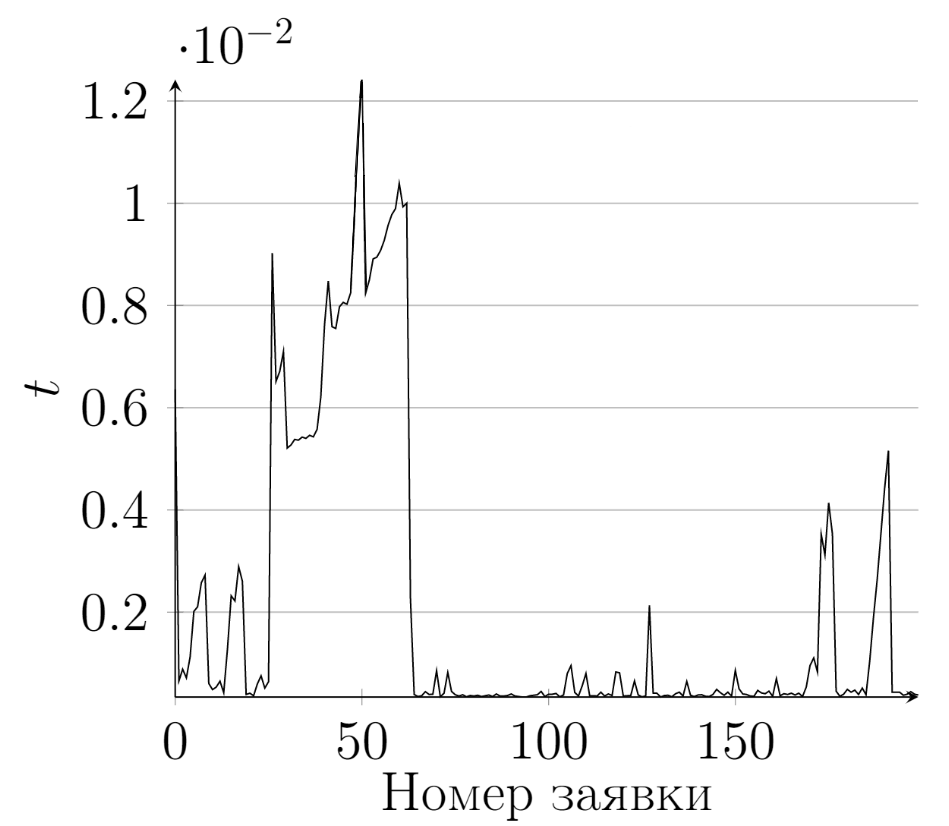
\includegraphics[scale=0.3]{graph_3q.png}}
	\caption{время проведённое заявкой в третьей очереди}
	\label{fig:image}
\end{figure}

\begin{figure}[h!]
	\center{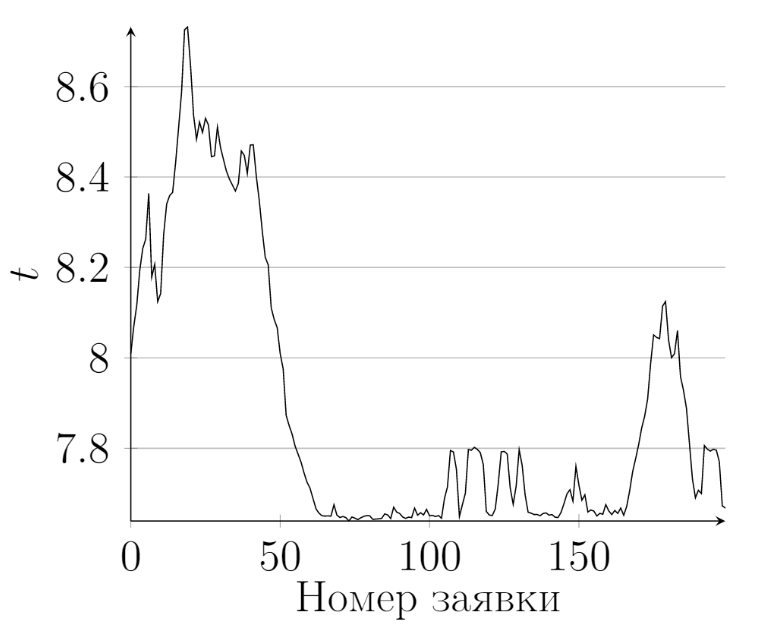
\includegraphics[scale=0.4]{graph_sum.png}}
	\caption{время проведённое заявкой в конвейере}
	\label{fig:image}
\end{figure}

Из графиков видно, что время нахождения во второй очереди резко растёт только в начале обработки, но затем 
спадает и держится на низком уровне.
В третьей очереди и всей системе наблюдается такая же картина, однако пики выше.\\

\newpage
В следующей таблице 4.1 приведены минимальные, максимальные и средние результаты замеренного времени в миллисекундах, 
проведённого заявками в очередях и во всём конвейере.

\begin{table}[h!]
	\caption{результаты проведённого заявками времени в очередях и системе}
	\label{tabular:timesandtenses}
	\begin{center}
		\begin{tabular}{ | l | l | l | l | l | l | l | }
			\hline
			& min               & max   & average \\ \hline
			Вторая очередь & $3 \cdot 10^{-4}$ & 0.739 & 0.140   \\ \hline
			Третья очередь & $3 \cdot 10^{-3}$ & 0.013 & 0.002   \\ \hline
			Система        & 7.753             & 8.732 & 7.890   \\ \hline
		\end{tabular}
	\end{center}
\end{table}

Можно сказать, что наибольшее время потрачено в ожидании поступления на конвейер, а значит первый этап 
является наиболее затратным по времени.

\section*{Вывод}
В данном разделе были рассмотрены результаты работы программы.
Из анализа стало ясно, что первый этап - шифрование с помощью шифра Цезаря замедляет работу всей системы, 
а также, что разница во времени работы 2 и 3 этапов крайне мала, что следует из малого времени, проведённого 
в третьей очереди.

\newpage
\chapter*{Заключение}
\addcontentsline{toc}{chapter}{Заключение}

В ходе лабораторной работы достигнута поставленная цель: разработка и исследование конвейерных вычислений и 
использование их на практике. 
Также решены все поставленные задачи.

Стало ясно, что шифрование Цезаря занимает достаточно большую часть времени обработки заявки, в то время как 
два XOR шифра выполняются с равной скоростью. Также стало ясно, что разделение основной задачи на этапы даёт 
положительный результат на общем времени работы программы. 



\newpage
\renewcommand\bibname{Список литературы}
\addcontentsline{toc}{chapter}{Список литературы}
\makeatletter % список литературы
\def\@biblabel#1{#1. }
\makeatother
\begin{thebibliography}{2}
	\bibitem{analyse_info} Дж. Макконнел. Анализ алгоритмов. Активный обучающий подход. -- М.: Техносфера, 2017. -- 267с.
	\bibitem{anatyse_info}Основы программирования на языках Си и C++ для начинающих[Электронный ресурс]. Режим доступа: http://cppstudio.com/ (дата обращения 10.10.2021)
	\bibitem{analyse_info}LINUX.ORG.RU - Русскоязычная информация о ОС Linux[Электронный ресурс] Режим доступа://www.linux.org.ru/(дата обращения 25.10.2021)
	\bibitem{analyse_info}  Документация языка C++ 98 [Электронный ресурс], режим доступа: http://www.open-std.org/JTC1/SC22/WG21/ (дата обращения 10.12.2021)
	\bibitem{} Р.А. Волков, А.Н. Гнутов, В.К. Дьячков и др. Конвейеры. Справочник. -Машиностроение, Ленинградское отделение, 1984.
	
\end{thebibliography}

\end{document}